%%%%%%%%%%%%%%% COPYRIGHT ANTOINE HUGOUNET & ETHEL VILLENEUVE
%%%%%%%%%%%%%%%%%%%%%%%%%%%%%%%%%%%%%%%%%%%%%%%%%%%%%%%
%%%%%%%%%%%%%%%%%%%%%%%%%%%%%%%%%%%%%%%%%%%%%%%%%%%%%%%


\documentclass[a4paper, twoside, 11pt]{report}

\usepackage[utf8]{inputenc}
\usepackage[T1]{fontenc}
\usepackage[english]{babel}
\usepackage[top= 120pt, left=80pt, right=80pt]{geometry} %marges
\usepackage{setspace} %interlignage
\usepackage{url}
\usepackage{graphicx}
\usepackage{lmodern} 
\usepackage{array}
\usepackage{csquotes}
\usepackage[numbers,square]{natbib}
\usepackage{soul}
\usepackage{hyperref}
\usepackage{amsthm}
\usepackage{color}
\usepackage[usenames,dvipsnames,svgnames,table]{xcolor}
\usepackage{adjustbox}
\usepackage{amssymb}
\usepackage{amsmath}
\usepackage{dsfont}
%%\usepackage{braket}
\usepackage{physics}
\usepackage{amsfonts}
\usepackage[numbers,square]{natbib}
\usepackage{multirow}
\usepackage{listings}
\usepackage{wasysym}

%%%%%% COULEURS CODE C++
\lstdefinestyle{customc}{
  belowcaptionskip=1\baselineskip,
  breaklines=true,
  frame=L,
  xleftmargin=\parindent,
  language=C,
  showstringspaces=false,
  basicstyle=\footnotesize\ttfamily,
  keywordstyle=\bfseries\color{red},
  commentstyle=\itshape\color{gray},
  identifierstyle=\color{NavyBlue},
  stringstyle=\color{black},
}

\lstdefinestyle{customasm}{
  belowcaptionskip=1\baselineskip,
  frame=L,
  xleftmargin=\parindent,
  language=[x86masm]Assembler,
  basicstyle=\footnotesize\ttfamily,
  commentstyle=\itshape\color{purple!40!black},
}

\lstset{escapechar=@,style=customc}

%%%%%% STYLES DE THÉORÈMES

\newtheoremstyle{theorem}%	Name
  {}%	Space above
  {}%	Space below
  {}%	Body font
  {}%	Indent amount
  {\bfseries}%	Theorem head font
  {.}%	Punctuation after theorem head
  { }%	Space after theorem head, ' ', or \newline
  {}%	Theorem head spec (can be left empty, meaning `normal')

\newtheoremstyle{exemple}%	Name
  {}%	Space above
  {}%	Space below
  {\color{Gray}\itshape}%	Body font
  {}%	Indent amount
  {\color{Gray}\itshape}%	Theorem head font
  {.}%	Punctuation after theorem head
  { }%	Space after theorem head, ' ', or \newline
  {}%	Theorem head spec (can be left empty, meaning `normal')

\newtheoremstyle{remark}%	Name
  {}%	Space above
  {}%	Space below
  {\itshape}%	Body font
  {}%	Indent amount
  {\bfseries}%	Theorem head font
  {.}%	Punctuation after theorem head
  { }%	Space after theorem head, ' ', or \newline
  {}%	Theorem head spec (can be left empty, meaning `normal')
  
%%%%%% DÉCLARATION DES THÉORÈMES

\theoremstyle{theorem}
\newtheorem{theorem}{Theorem}[section]
\newtheorem{lemme}{Lemma}[section]
\newtheorem{proposition}{Proposition}[section]
\newtheorem{definition}{Definition}[section]

\theoremstyle{remark}
\newtheorem{remark}{Remark}[chapter]

\theoremstyle{exemple}
\newtheorem*{exemple}{Example}


%%%%%% COMMANDES QUI SIMPLIFIENT LA VIE

\newcommand{\legende}[1]{
\begin{center}
	\begin{minipage}{12cm}
		\begin{center}
			\textit{\textcolor{WildStrawberry!30}{#1}}
		\end{center}
	\end{minipage}
\end{center}}

\newcommand{\sherlock}[2]{
	\begin{equation}
		\textcolor{WildStrawberry}{#1}
	\end{equation}
	\legende{#2}
}
	
\newcommand{\sherlocked}[1]{
	\begin{equation}
		\textcolor{WildStrawberry}{#1}
	\end{equation}
}

	
\newcommand{\defSherlock}[3]{
	\begin{definition}[\textbf{#1}]
		\sherlock{#2}{#3}
	\end{definition}
}

\newcommand{\defSherlocked}[2]{
	\begin{definition}[\textbf{#1}]
		\sherlocked{#2}
	\end{definition}
}	

\newcommand{\propSherlock}[3]{
	\begin{proposition}[\textbf{#1}]
		\sherlock{#2}{#3}
	\end{proposition}
}

\newcommand{\propSherlocked}[2]{
	\begin{proposition}[\textbf{#1}]
		\sherlocked{#2}
	\end{proposition}
}

\newcommand{\textSherlocked}[1]{
	\begin{center}
		\textcolor{WildStrawberry}{#1}
	\end{center}
}

\newcommand{\N}{\mathbb{N}}
\newcommand{\Z}{\mathbb{Z}}
\newcommand{\R}{\mathbb{R}}
\newcommand{\C}{\mathbb{C}}


%%%%%%%%%%%%%%%%%%%%%%%%%%%%%%%%%%%%%%%%%%%%%%%%%%%%%%%
%%%%%%%%%%%%%%%%%%%%%%%%%%%%%%%%%%%%%%%%%%%%%%%%%%%%%%%
%%%%%%%%%%%%%%%%%%%%%%%%%%%%%%%%%%%%%%%%%%%%%%%%%%%%%%%

\title{FYS3150\\Project 3 - The Verlet Underground}
\author{Hugounet, Antoine \& Villeneuve, Ethel}
\date{September 2017 \\University of Oslo \\ \url{https://github.com/kryzar/Perseids.git}}



\begin{document}
\selectlanguage{english}
\maketitle
	
	
\begin{abstract}

	\paragraph{}The aim of this project is to create a simulation of the Solar System. We will consider three cases.
		\begin{enumerate}
			\item{The first one will be the simplest, an Earth-Sun system. With it, we can test our program and compare the Euler's and Verlet's method as we know that the orbit of the Earth is supposed to be circular around the Sun, which will be set as the center-of-mass.}
			\item{In the second case, we will add Jupiter. With this model, we can compare the influence of taking into account the real center-of-mass instead of the Sun as center-of-mass.}
			\item{Finally, the third case will be the complete Solar System (without moons, only the eight planets). After checking that our program is stable and viable, we can simulate the Solar System around the years and centuries.}
		\end{enumerate}
		
	Moreover, we will use the program to find the escape value of the Earth from the Sun and to study the Mercury's perihelion precession with and without a relativistic correction to Newton's law. These are two concrete ways to use this simulation program, but it basically works for many phenomena.
	
	\paragraph{}As we expected, Verlet's method is way more precise than Euler's method. That is why we will use Euler's one only for the two-bodies model. In contrast, changing the center-of-mass from the Sun to the real one does not implies big changes as it is really close to the Sun compared to the other distances.  
	
\end{abstract}


\tableofcontents


\chapter*{Introduction}
\addcontentsline{toc}{chapter}{Introduction}

    \paragraph{}
    

\chapter{Theory}
    
    \paragraph{}In a first place, we will begin with an Earth-Sun system with the Earth orbiting around the Sun. We will test our simulation on this simple case and add the other planets afterwards. 

    \section{Earth-Sun system}
    
        \subsection{Physical conditions of the system}
        
            \paragraph{}The only force applied to this system is the gravity. According to the Newton's law, we have 
                \begin{equation}
                F_G = \frac{GM_{\odot}M_{\oplus}}{r^2}
                \end{equation}
            with $F_G$ the norm of the gravitational force, $G$ the gravitational constant ($G=6.674 \times 10^{-11} \mathrm{N}.\mathrm{m}^2.\mathrm{kg}^{-2}$), $M_{\odot}$ the mass of the Sun, $M_{\oplus}$ the mass of the Earth and $r$ the distance between the Earth and the Sun.\\
            We will neglect the motion of the Sun here as the mass of the Sun is much larger than the mass of the Earth ($M_{\odot} = 2 \times 10^{30}$kg against $M_{\oplus} = 6 \times 10^{24}$kg). We want to establish the motion of the Earth around the Sun. Moreover, we will assume that the orbit of the Earth around the Sun is coplanar in the $xy$-plane.
            \paragraph{}The Newton's second law of motion states that the total force applied to any system in a Galilean referential is $\overrightarrow{F}=M\overrightarrow{a}$ with $M$ the mass of the body concerned and $\overrightarrow {a}$ the acceleration. Applied to our case, we have $\overrightarrow{{F}_{G}} = {M}_{\oplus} \overrightarrow{a}$. Since $a$ is the second derivative of the position : 
                \begin{align*}
                    F_{G,x} &= M_{\oplus} \frac{d^2 x}{dt^2} \\
                    F_{G,y} &= M_{\oplus} \frac{d^2 y}{dt^2}
                \end{align*}
            or
                \begin{align}
                    \frac{d^2 x}{dt^2} &= \frac{F_{G,x}}{M_{\oplus}} \tag{1}\\
                    \frac{d^2 y}{dt^2} &= \frac{F_{G,y}}{M_{\oplus}} \tag{2}.
                \end{align}
            with $F_{G,x}$ and $F_{G,y}$ the components of the gravitational force.\\
            \begin{remark}
            	We will not use the SI units but the Astronomical units (AU) for the distances (with $1$AU$=$average distance Earth-Sun $=1.5 \times 10^{11}$m), kg for masses and years for time units. Thus the initial position of the Earth will be $x_{\oplus} = 1$, \hspace{0,1cm}$y_{\oplus} = 0$ with the Sun the origin ($x_{\odot} = 0$, $y_{\odot} = 0$). 

			\end{remark}
            To simplify a little bit, we will assume that the Earth's orbit is circular around the Sun. So we can write :
                \begin{equation}
                    F_G = \frac{M_{\oplus} v^2}{r} = \frac{GM_{\odot}M_{\oplus}}{r^2}
                    \tag{3}
                \end{equation}
            with $v$ the velocity of Earth. From here we have
                \begin{equation*}
                    v^2 r = GM_{\odot} = 4 \pi^2 \mathrm{AU}^3 / \mathrm{yr}^2
                    \tag{4}
                \end{equation*}
            
        \subsection{Escape velocity}
        
            \paragraph{}In the case where only the gravitational force is applied, the mechanical energy $E_m = E_c + E_p$ with $E_c$ the kinetic energy and $E_p$ the potential energy is conserved (the gravitational force is conservative). For a planet at a distance of 1 AU from the Sun (let's take the Earth as an example), the kinetic energy is given by $E_c = \frac{1}{2}M_{\oplus}\times v^2$ and the potential energy by $E_p = - \frac{G M_{\odot} M_{\oplus}}{r}$ with $r=1$ AU. 
            \\We want this planet to escape from the gravitational attraction of the Sun on it. The escape velocity will be the minimal speed $v_e$ at which the planet escapes from the gravitational influence of the Sun. We consider two positions of the planet : $p_i$ the initial position when $r_i=1$AU and $p_f$ the final position when the planet has escaped and is at an infinite distance from the Sun $r_f=\infty$.
            
            \paragraph{}Let's consider the mechanical energy at the final position. We have $E_{m_f} = E_{c_f} + E_{p_f}$, $E_{c_f} = 0$ as the velocity of the planet is zero at the final state, $E_{p_f}=0$ since $r_f=\infty$ and $E_{m_f}=0$. \\
            So, with the planet at 1 AU from the Sun at its inital position, of which velocity is the escape velocity $v_e$, in the case where there is only the gravitational force applied to the system planet-Sun, we have :
                \begin{equation*}
                    E_{c_i} + E_{p_i} = \frac{1}{2}M_{\oplus} \times v_e^2 - \frac{GM_{\odot}M_{\oplus}}{r_i} = E_{c_f} + E_{p_f} = 0
                \end{equation*}
            according to the law of conservation of energy. From this we can write
                \begin{align*}
                    \frac{1}{2}M_{\oplus} \times v_e^2 &- \frac{GM_{\odot}M_{\oplus}}{r_i} = 0 \\
                    \Rightarrow v_e &= \sqrt{\frac{2GM_{\odot}}{r_i}} \\
                    \Rightarrow v_e &=\sqrt{2GM_{\odot}}
                \end{align*}
            which only depends on the mass of the Sun. 
                \begin{align*}
                    v_e &= \sqrt{2\times 4\pi^2}, \hspace{0.5cm} \mathrm{from (4)}\\
                    v_e &= 2\sqrt{2}\pi \hspace{0.2cm} \mathrm{AU/yr}
                \end{align*}
            Then, for a velocity $v \geq 2\sqrt{2}\pi$, the Earth would escape from the Sun's gravitational attraction. 
                        
                        
    
    \section{Three-body problem}
        \paragraph{}We add Jupiter to the previous system and place it on the same $x-axis$ that the Earth is on. In the previous case, the Earth's motion was a stable circular orbit in time. Adding Jupiter, it will inevitably be disturbed.
        
        \paragraph{}We can write the gravitational between the Earth and Jupiter as 
                \begin{equation*}
                    F_{\oplus-\jupiter} = \frac{GM_{\jupiter}M_{\oplus}}{r_{\oplus-\jupiter}^2} 
                \end{equation*}
            with $M_{\jupiter}$ the mass of Jupiter and $r_{\oplus - \jupiter}$ the distance between the Earth and Jupiter. \\
            The algorithm used for this case will be exactly the same as the previous case. We will see in section 1.4 how to discretize and implement the algorithm. 
            
        \subsection{Real center-of-mass}
        
            \paragraph{}To get closer to the reality, we now do not consider the Sun as a static body anymore ; each of three bodies are in motion and considered as planets. The center-of-mass will not be the Sun but the real one. Let's compute the new coordinates of the celestial bodies.
            
            \subsubsection{Basic equation}
            
                \begin{equation}
                    \left\{
                        \begin{aligned}
                    x_c &= \frac{1}{M_{tot}}\sum\limits_{i} M_i x_i\\
                    y_c &= \frac{1}{M_{tot}}\sum\limits_{i} M_i y_i
                \end{aligned}
                    \right.
                \end{equation} 
            
            Considering the system Earth-Jupiter-Sun :
            
                \begin{align*}
                    M_{tot} &= M_{\oplus} + M_{\jupiter} + M_{\odot} \\
                    &= 6\times10^{24} + 1.9\times 10^{27} + 2 \times 10^{30}\\
                    &= 2.00191 \times 10^{30} \mathrm{kg}
                \end{align*}
                \begin{equation*}
                    \left\{
                        \begin{aligned}
                            x_c = \frac{1}{M_{tot}} [M_{\oplus} x_{\oplus_i} + M_{\jupiter} x_{\jupiter_i} + M_{\odot} x_{\odot_i}] \\
                            y_c = \frac{1}{M_{tot}} [M_{\oplus} y_{\oplus_i} + M_{\jupiter} y_{\jupiter_i} + M_{\odot} y_{\odot_i}]
                        \end{aligned}
                    \right.
                \end{equation*} 
            We fix the initial positions with respect to the new center of mass.
            
            \subsubsection{Calculations}
            
                \begin{center}
                \begin{figure}[h!]
                    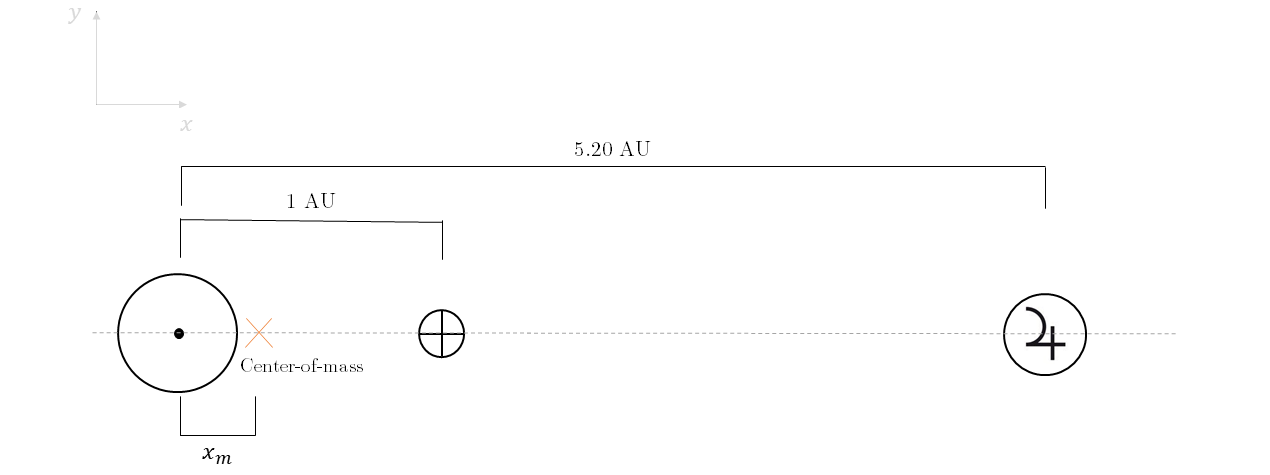
\includegraphics[width=16cm,height=6cm]{dessinplanete.png}
                    \caption{Representation of the initial position of our three-bodies system.}
                \end{figure}
                \end{center}
                
            So we look for $x_m$ the $x$-component of the position of the Sun such that $x_c=y_c=0$.
            
                \begin{equation*}
                    \left\{
                        \begin{aligned}
                            x_c &= \frac{1}{M_{tot}} [(2 \times 10^{24}) \times (1 + x_m) + (1.9 \times 10^{27}) \times (5.20 + x_m) + (2 \times 10^{30}) \times x_m] = 0 \\
                            y_c &= 0 
                        \end{aligned}
                    \right.
                \end{equation*}
                
                \begin{equation*}
                    \Longrightarrow \left\{ 
                        \begin{aligned}
                            x_m &= -4.936 \times 10^{-3}\\
                            y_m &= 0
                        \end{aligned}
                    \right.
                    \tag{5}
                \end{equation*}
            These are the coordinates of the Sun when the center-of-mass of the system is set as the origin. Let's now compute the Sun's initial velocity such that the total momentum of the three-body system equals 0.
                \begin{equation}
                    \overrightarrow{p_{tot}} = \sum\limits_{k} M_k \overrightarrow{k} = \overrightarrow{0} \\
                \end{equation}
                
                \begin{equation*}
                    \Longrightarrow \left(\begin{array}{c}
                            0\\
                            0
                    \end{array} \right) = M_{\oplus} 
                        \left(\begin{array}{c}
                                v_{\oplus_x}\\
                                v_{\oplus_y}
                        \end{array} \right) + M_{\jupiter}
                             \left(\begin{array}{c}
                                    v_{\jupiter_x}\\
                                    v_{\jupiter_y}
                            \end{array} \right) + M_{\odot}
                                \left(\begin{array}{c}
                                        v_x\\
                                        v_y    
                                \end{array} \right)
                \end{equation*}
                \begin{equation*}
                   \Longrightarrow \left\{
                        \begin{aligned}
                            M_{\oplus} v_{\oplus_x} + M_{\jupiter} v_{\jupiter_x} + M_{\odot} v_x = 0 \\
                            M_{\oplus} v_{\oplus_y} + M_{\jupiter} v_{\jupiter_y} + M_{\odot} v_y = 0
                        \end{aligned}
                    \right.
                \end{equation*}
            
            \paragraph{}We choose the initial velocities of the Earth and Jupiter so that their orbit will be circular.\\
            If the orbit of the Earth is circular around the center-of-mass, $v_{\oplus} = 2 \pi \times (1+x_m)$ AU/yr, because the distance travelled in one Earth-year is $2 \pi \times r$ with $r = 1 + x_m$ AU.
            
            \paragraph{}Similarly $v_{\oplus} = 6.25217$ AU/yr. The velocity is constant so the initial velocity will be $v_{\oplus_i}=6.25217$ AU/yr. In the initial configuration represented above, the initial velocity is oriented in the direction of $y$. So, $v_{\oplus_i} = \left(0, 6.25217\right)$. \\
            Jupiter has an orbital period of $11.862$ yr. The distance travelled by Jupiter in this period is $2 \pi \times r = 2 \pi \times (5.20 + x_m) = 32.6415 AU$. So $v_{\jupiter_i}= \frac{2 \pi \times r}{T} = \frac{2 \pi \times (5.20+x_m)}{11.862} = 2.75177 $ AU/yr. Similarly, the initial velocity can be expressed as $v_{\jupiter_i} = \left(0, 2.75177\right)$.
            
                \begin{equation*}
                    \left\{
                        \begin{aligned}
                            &(6\times 10^{24}) \times 0 + (1.9 \times 10^{27}) \times 0 + (2 \times 10^{30}) \times v_x = 0 \\
                            &(6\times 10^{24}) \times 6.25217 + (1.9 \times 10^{27}) \times 2.75177 + (2 \times 10^{30}) \times v_y = 0
                        \end{aligned}
                    \right.
                \end{equation*}.
                \begin{equation*}
                   \Longrightarrow \left\{
                        \begin{aligned}
                            v_x &= 0\\
                            v_y &= - 2.63294 \times 10^{-3}
                        \end{aligned}
                    \right.
                    \tag{6}
                \end{equation*}
            \paragraph{}Therefore, our initial vectors will be :
            \begin{center}           
                \begin{tabular}{|c|c|c|}
                        \hline
                    Body & Position & Velocity \\
                        \hline
                    Earth & $\left(\begin{array}{c}
                        0.995064 \\
                        0
                        \end{array}\right)$ 
                        & $\left(\begin{array}{c}
                        0 \\
                        6.25217
                        \end{array}\right)$\\
                        \hline
                    Jupiter & $\left(\begin{array}{c}
                        5.19506 \\
                        0
                        \end{array}\right)$ 
                        & $\left(\begin{array}{c}
                        0 \\
                        2.75177
                        \end{array}\right)$\\
                        \hline
                    Sun & $\left(\begin{array}{c}
                        -4.936 \times 10^{-3} \\
                        0
                        \end{array}\right)$ 
                        & $\left(\begin{array}{c}
                        0 \\
                        -2.63294 \times 10^{-3}
                        \end{array}\right)$ \\
                        \hline
                \end{tabular}
            \end{center}

    \section{The complete Solar system}
        \paragraph{}As the program had been made so that we can add as many planets as we want, modelizing the complete Solar System is not more complicated than having only the system Earth-Jupiter-Sun. We will take, in that case, the center-of-mass of the complete Solar System as origin. Therefore the Sun has a motion.
        

    \subsection{Discretization}
    
    \paragraph{}The discretization is a crucial step to make the equations "understandable" by our program. From Newton's law of motion, the acceleration of a given body can be written as $a=\frac{F_G}{M}$, with $M$ the mass of the body. $a_i$ is the acceleration at the time $t_i$, and ${a}_{i+1}$ is the very next discretized value of the acceleration at ${t}_{i+1}={t}_{i}+h$.
                \begin{equation*}
                    a_i = \frac{ \sum\limits_{k} \frac{GMM_{k_N}}{r_{i_k}^2}}{M}
                \end{equation*}
            with $k$ the number of bodies involved in the system. 
                \begin{equation*}
                    a_i = \sum\limits_{k} \frac{GM_{k_N}}{r_{i_k}^2}
                \end{equation*}
            From (4), we have $GM_{\odot} = 4\pi^2\mathrm{AU}^3/\mathrm{yr}^2$ and as $M_{\odot}=1$, $G=4\pi^2\mathrm{AU}^3/\mathrm{yr}^2$. So,
                \begin{align*}
                    a_i &= \sum\limits_{k} \frac{4\pi^2M_{k_N}}{r_{i_k}^2} \\
                    a_i &= \sum\limits_{k} \frac{4\pi^2M_{k_N}(x_i-x_{i_k})}{r_{i_k}^3} 
                    \tag{7}
                 \end{align*}
                 
                     \begin{remark}
    	To implement the accelerations, we normalize the masses with respect to the mass of the Sun. Thus, $M_{\odot}=1$, $M_{k_N}=\frac{M_k}{M_{\odot}}$ is the normalized mass for each body $k$. We use $AU$ as the distance unit and the year $yr$ as the time unit.
	\end{remark}
        \subsection{Euler's method}
            
             With Euler's method, we simply compute the derivation formula for a supposed small constant time-step $h$ : $\displaystyle a_i = \frac{d{v}_{i}}{dt}=\frac{v_{i+1} - v_i}{h}$. With $\displaystyle h = \frac{b-a}{N}$ and $N$ the number of time-steps, the bigger $N$, the smaller $h$, and the more accurate Euler's approximation is.
             
             \begin{remark}
             	It is easier to see this formula as the formula of the derivative without its limit, but Euler's demonstrated it in terms of Taylor's expansion.
			\end{remark}
			 
                \begin{align*}
                     &\frac{v_{i+1} - v_i}{h} = \sum\limits_{k}\frac{4\pi^2M_k(x_i-x_{i_k})}{r_{i_k}^3} \\
                     \Longrightarrow &v_{i+1} = h\sum\limits_{k}\frac{4\pi^2M_k(x_i-x_{i_k})}{r_{i_k}^3} + v_i
                    \tag{8}
                \end{align*}
             \paragraph{}The velocity can also be discretized as the derivative of the position
                \begin{equation*}
                      v_i = \frac{x_{i+1}-x_i}{h}
                  \end{equation*}
             Therefore,
                 \begin{equation*}
                    x_{i+1} = hv_i + x_i
                    \tag{9}
                \end{equation*}   
            The initial position and velocity of the body are obtained with the data from the NASA website.
            
        \subsection{Verlet's method}
            \paragraph{}Verlet's method is almost the same as the Euler's one in the sense that it is based on Taylor's expansion, but goes one step further. We consider two instants $t_i+h$ as $t_i-h$ :
                \begin{equation*}
                    \left\{ 
                        \begin{aligned}
                            x_{i+1} &= x(t_i+h) = x(t_i) + h\frac{dx}{dt}(t_i) + \frac{h^2}{2!}\frac{d^2x}{dt^2}(t_i) + \frac{h^3}{3!}\frac{d^3x}{dt^3}(t_i)+\mathcal{O}(h^4)\\
                            x_{i-1} &= x(t_i-h) = x(t_i) - h\frac{dx}{dt}(t_i) + \frac{h^2}{2!}\frac{d^2x}{dt^2}(t_i) - \frac{h^3}{3!}\frac{d^3x}{dt^3}(t_i)+\mathcal{O}(h^4)
                        \end{aligned}
                    \right.
                \end{equation*}
            We sum up the two lines to have
                \begin{align*}
                    x_{i+1} &+ x_{i-1} = 2x_i + h^2\frac{d^2x_i}{dt^2} + \mathcal{O}(h^4) \\
                    \Rightarrow x_{i+1} &= 2x_i - x_{i-1} + h^2\frac{d^2x_i}{dt^2} + \mathcal{O}(h^4)
                \end{align*}
            \paragraph{}Another way to use the Verlet's method is with :
                \begin{equation*}
                    \left\{
                        \begin{aligned}
                            x_{i+1}&=x(t_i+h) = x(t_i) + h\frac{dx}{dt}(t_i) + \frac{1}{2}h^2 \frac{d^2x}{dt^2}(t_i)\\
                            v_{i+1}&=v(t_i+h) = v(t_i) + \frac{1}{2}h(\frac{dv}{dt}(t_i) + \frac{dv}{dt}(t_i+h)
                        \end{aligned}
                    \right.
                \end{equation*}
            where the velocity is explicitly expressed.
            


\chapter{Implementation}

    \section{Earth-Sun system}
        \subsection{}
        
        \subsection{Tests}
            \paragraph{}The mechanical energy $E_m = E_c + E_p$ should be conserved because the only force taken into account is the gravitational force, which is conservative. The potential energy is constant in time ($E_p = -\frac{GM_{\oplus}M_{\odot}}{r} \forall t$), so is conserved. The kinetic energy depends on the velocity of the Earth ($E_c = \frac{1}{2}M_{\oplus}v^2$, which is constant in time as we have a uniform circular motion of the Earth around the Sun. So as both of the kinetic and potential energies are constant in time, for any $t_i$ and $t_f$ we have
                \begin{equation*}
                    \left\{
                        \begin{aligned}
                            E_{c_i} &= E_{p_f}\\
                            E_{p_i} &= E_{p_f}
                        \end{aligned}
                    \right. \hspace{0.5cm} \Rightarrow E_{c_i} + E_{p_i} = E_{c_f} + E_{p_f}
                \end{equation*} 
                \begin{equation*}
                    \Rightarrow E_{m_i} = E_{m_f}
                \end{equation*}
                        
    
    \section{Adding one planet}
    
    
    \section{The complete Solar system}
    
    

\chapter{Results}
    \section{Earth-Sun system}
        \subsection{Comparison between the two algorithms}
            \paragraph{}Let's compare the results between using the Euler's method and the Verlet's method.
                \begin{figure}[h]
                    \hbox{
                        \begin{minipage}[c]{.30\linewidth}
                            \centering
                            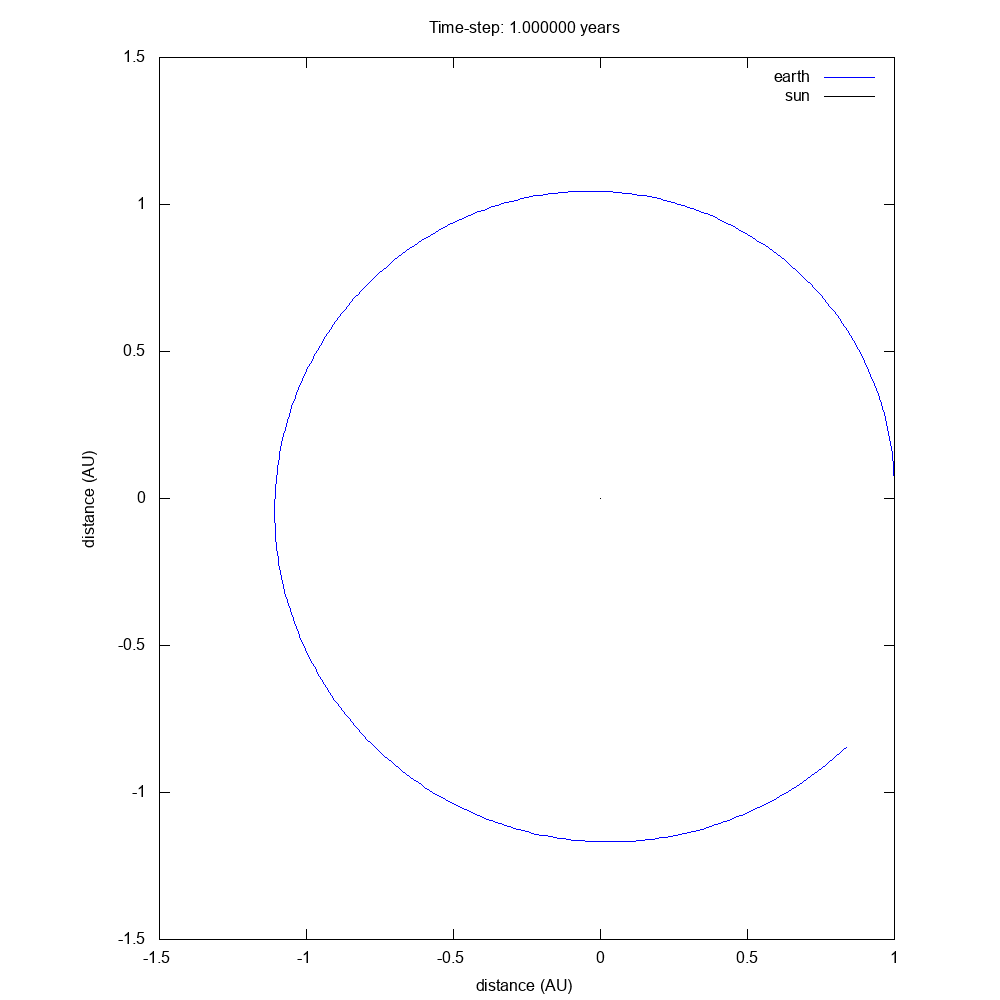
\includegraphics[width=5.5cm,height=4.5cm]{Euler1.png}
                            \caption{Euler's method over 1 year}
                        \end{minipage}
                        \hspace{1mm}
                        \begin{minipage}[c]{.30\linewidth}
                            \centering
                            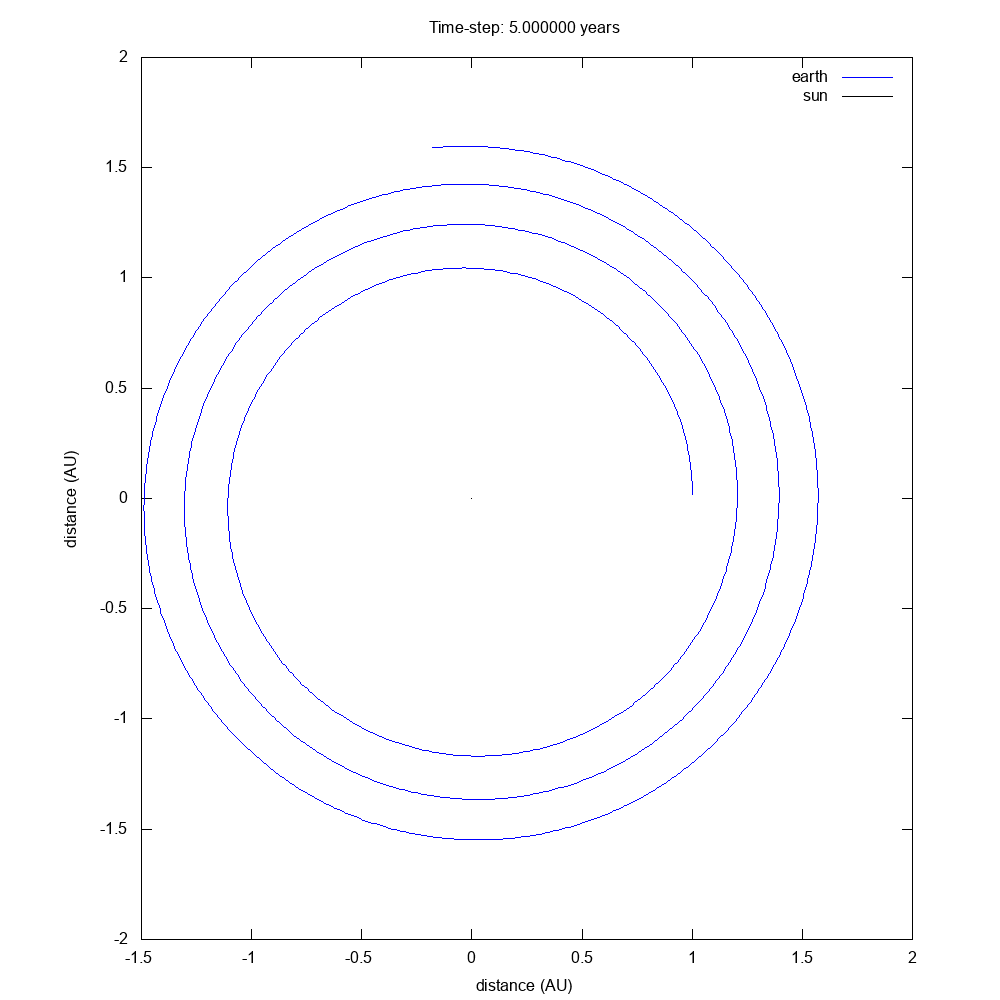
\includegraphics[width=5.5cm,height=4.5cm]{Euler2.png}
                            \caption{Euler's method over 2 years}
                        \end{minipage}
                        \hspace{2.5mm}
                        \begin{minipage}[c]{.30\linewidth}
                            \centering
                            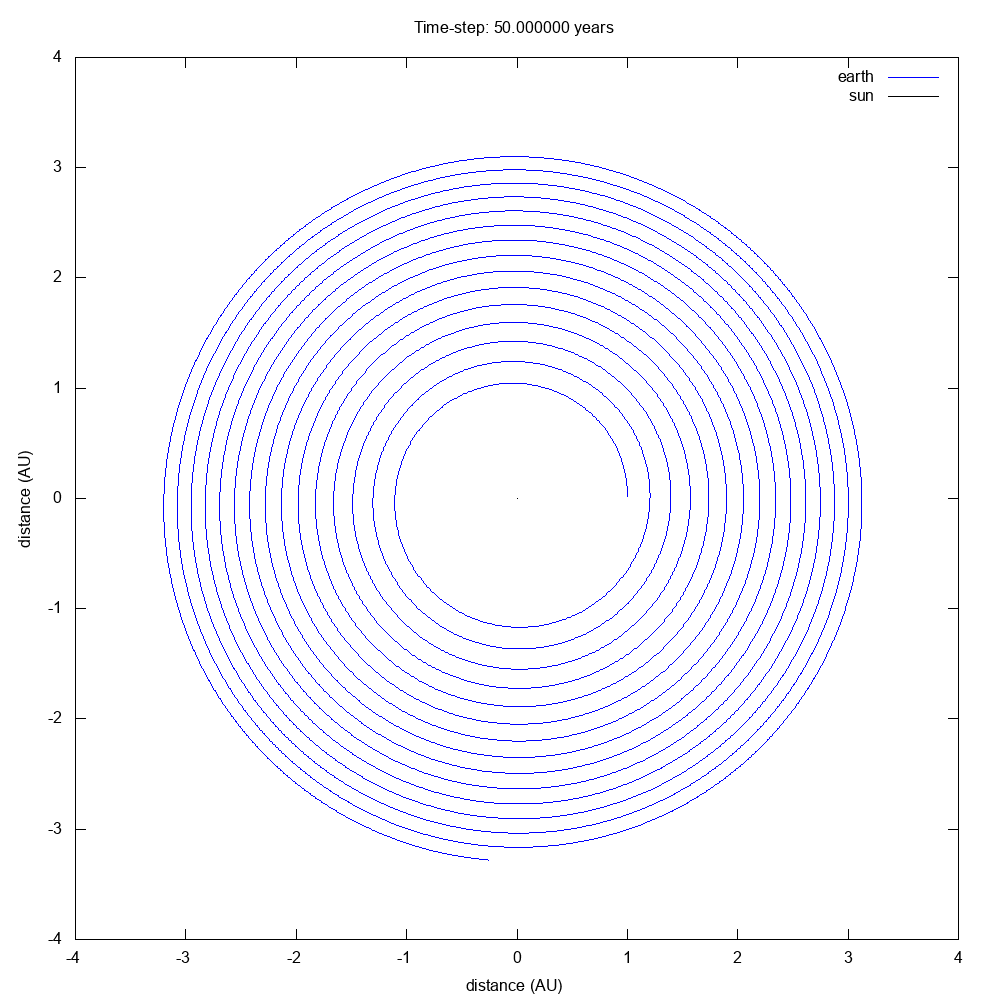
\includegraphics[width=5.5cm,height=4.5cm]{Euler50.png} 
                            \caption{Euler's method over 50 years}   
                        \end{minipage}
                    }
                \end{figure}
                \begin{figure}[h]
                    \hbox{
                        \begin{minipage}[c]{.30\linewidth}
                            \centering
                            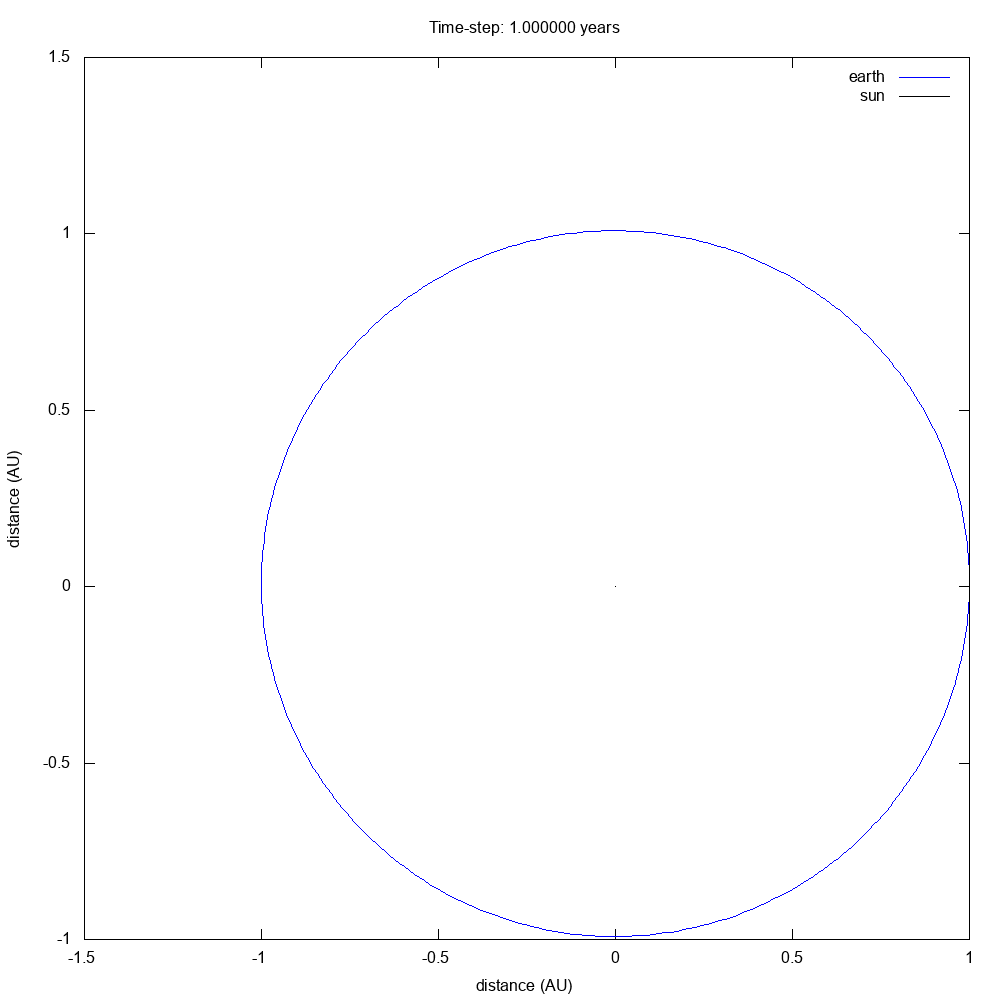
\includegraphics[width=5cm,height=4.5cm]{Verlet1.png}
                            \caption{Verlet's method over 1 year}
                        \end{minipage}
                        \hspace{1mm}
                        \begin{minipage}[c]{.30\linewidth}
                            \centering
                            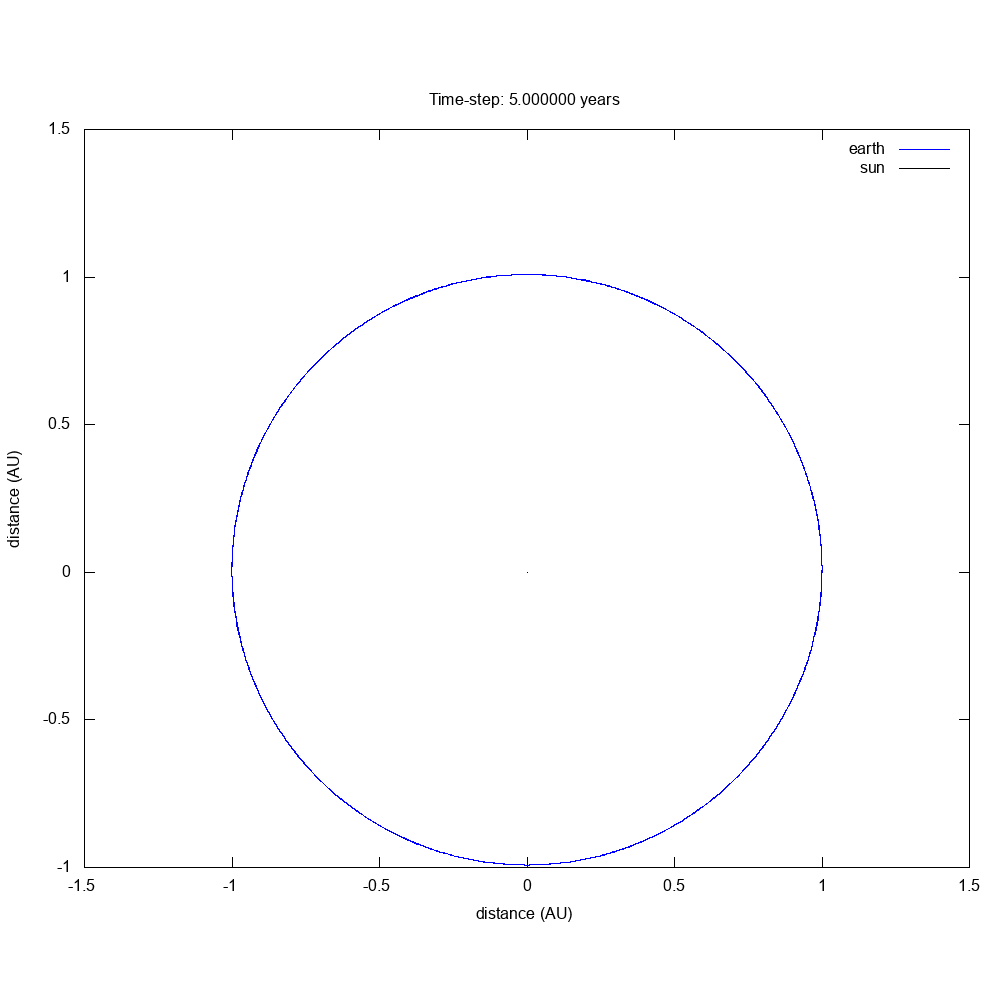
\includegraphics[width=5cm,height=4.6cm]{Verlet2.png}
                            \caption{Verlet's method over 2 years}
                        \end{minipage}
                        \hspace{2.5mm}
                        \begin{minipage}[c]{.30\linewidth}
                            \centering
                            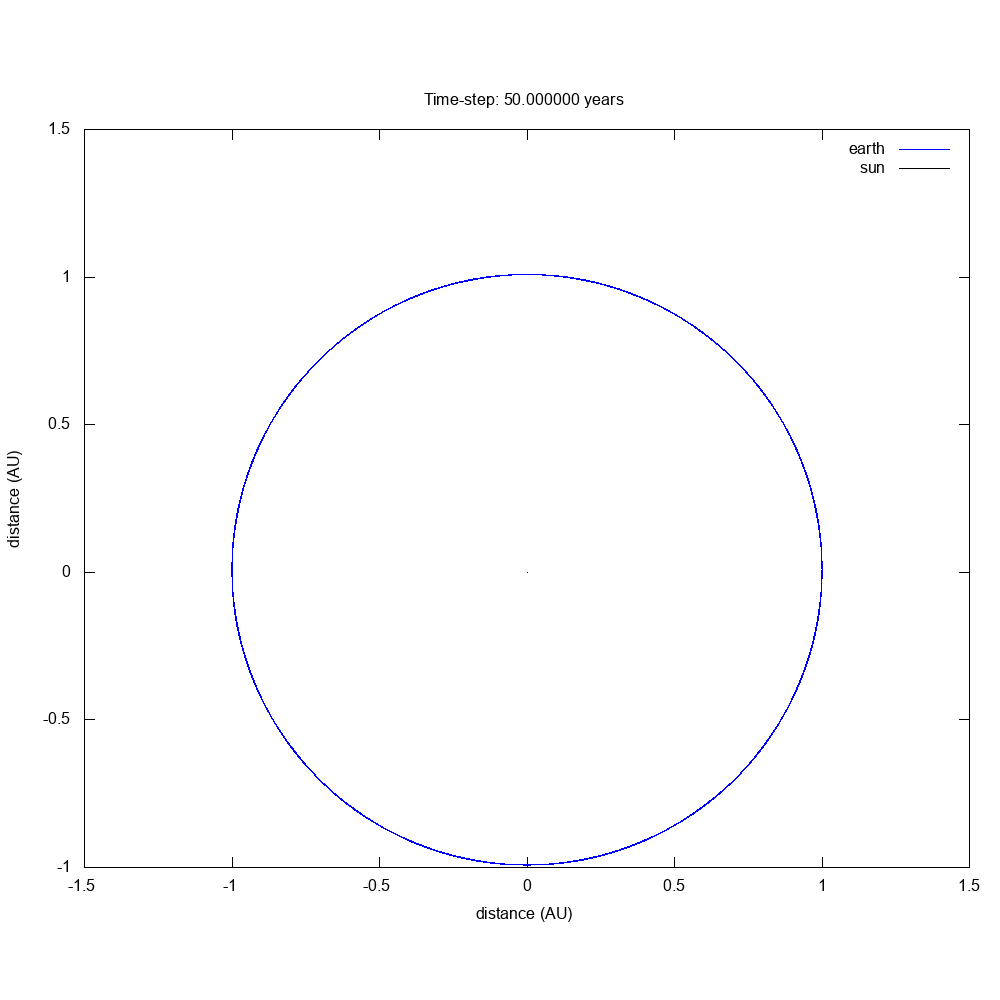
\includegraphics[width=5cm,height=4.6cm]{Verlet50.png} 
                            \caption{Verlet's method over 50 years}   
                        \end{minipage}
                    }
                \end{figure}
            We clearly see here the difference of precision between the two algorithms. With the Euler's method, the Earth is not able to come back at its initial position as it should whereas the Verlet's one draws a circular orbit.
        
        \subsection{Escape velocity}
            \paragraph{}We have computed the theorical escape velocity in 1.1.2.
                \begin{figure}[h]
                    \hbox{
                        \begin{minipage}[c]{.46\linewidth}
                            \centering
                            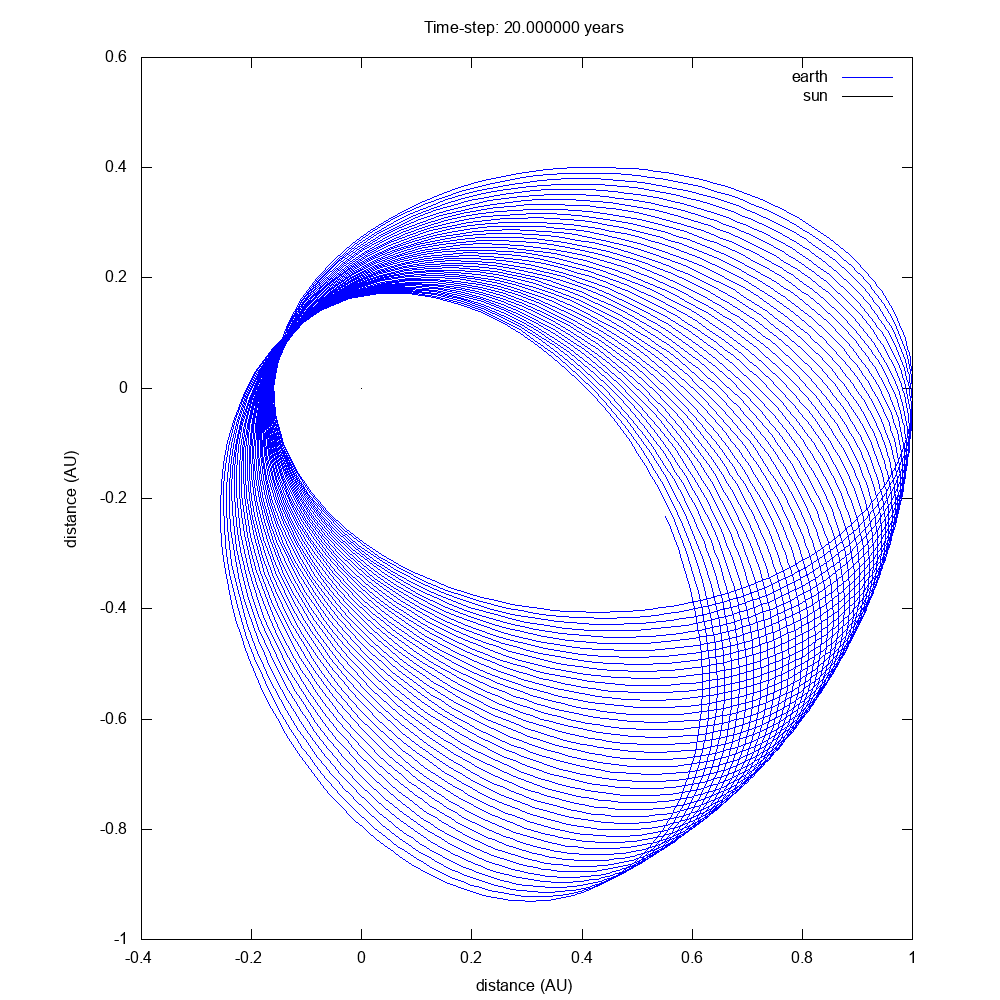
\includegraphics[width=7cm,height=7cm]{Escape0,009.png}
                            \caption{Earth orbit for $v_i=3.287$ AU/yr}
                        \end{minipage}
                        \hfill
                        \begin{minipage}[c]{.46\linewidth}
                            \centering
                            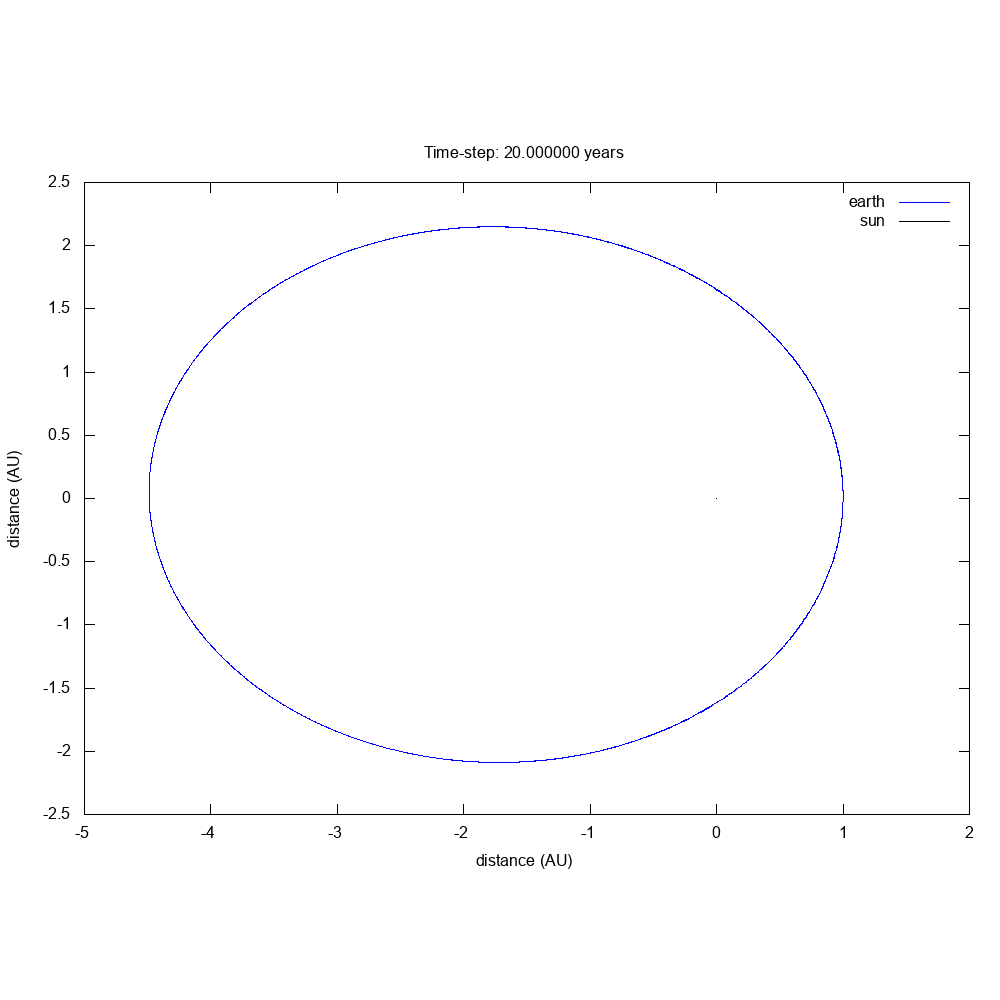
\includegraphics[width=7cm,height=7cm]{Escape0,022.png}
                            \caption{Earth orbit for $v_i=8.0355$ AU/yr}
                        \end{minipage}
                    }
                \end{figure}
                \begin{figure}[h]
                    \hbox{
                        %\begin{minipage}[c]{.46\linewidth}
                           % \centering
                           % \includegraphics[width=7cm,height=7cm]{Escape0,024}
                         %   \caption{Earth orbit for $v_i=8.77$ AU/yr}
                       % \end{minipage}
                       % \hfill
                        \begin{minipage}[c]{.46\linewidth}
                            \centering
                            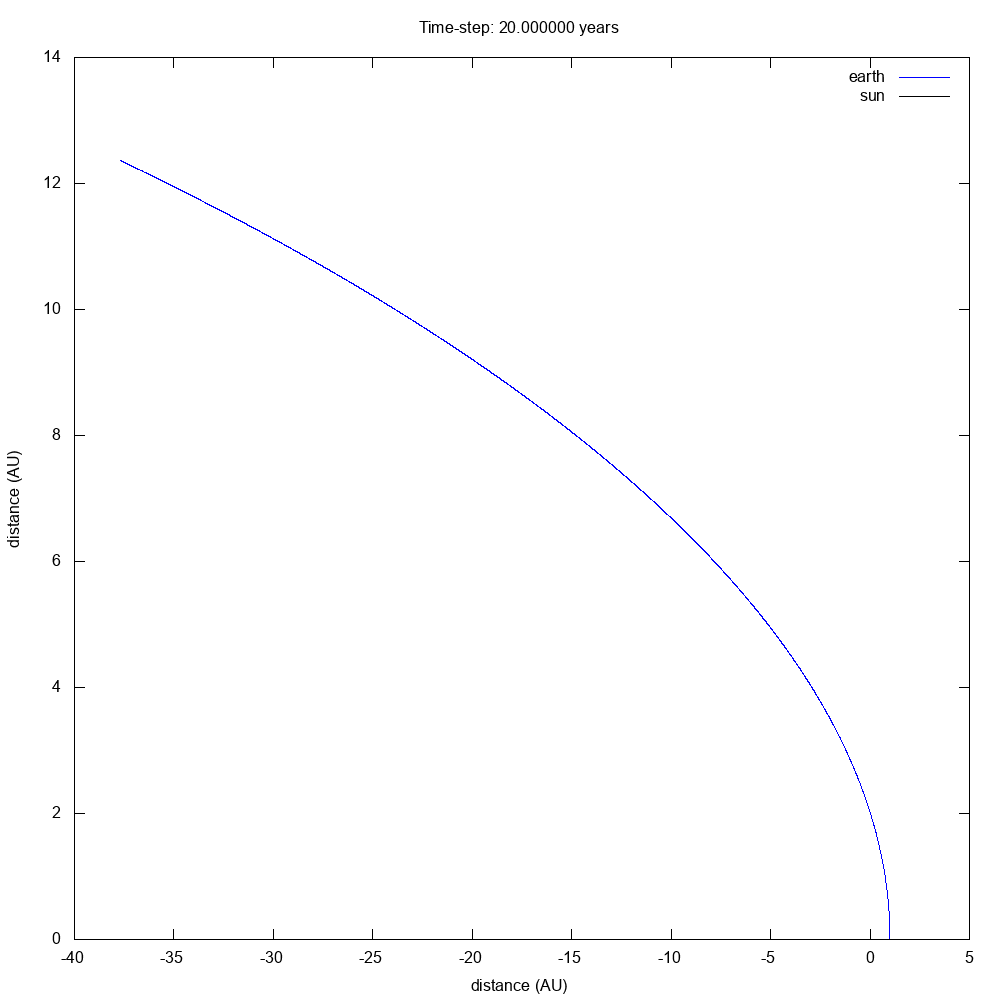
\includegraphics[width=7cm,height=7cm]{Escape0,0243.png}
                            \caption{Earth orbit for $v_i=8.8756$ AU/yr}
                        \end{minipage}
                    }
                \end{figure}
    
    \section{Three-body problem}
        \subsection{The Sun as the center-of-mass}
        
        \subsection{The real center-of-mass}
    
    
    \section{Complete Solar System}
        \subsection{}
        
        \subsection{}
    
    

\chapter*{Conclusion}
\addcontentsline{toc}{chapter}{Conclusion}

    \paragraph{}
    
    
    
    
\chapter*{Bibliography}
    \begin{itemize}
        \item NASA website \href{{http://ssd.jpl.nasa.gov/horizons.cgi#top}}{\nolinkurl{http://ssd.jpl.nasa.gov/horizons.cgi\#top}}
        \item 
    \end{itemize}
    
    
    
    
    
    
    
    
    
    
\end{document}